% tex file for future discussion
\par \indent The implementation of permutation tests, which have few 
assumptions and are easy to interpret (but computationally intensive), 
would have been useful for testing the significance of the estimated 
coefficients from linear modeling as an alternative to t-tests, which make 
several assumptsion about the data structure. Somewhat relatedly, 
additional tests and checks for model assumptions would also be valuable 
for assessing the appropriateness of our existing hypothesis testing. 

\par One major issue that we were unable to fully address is how to 
appropriately aggregate the results from individual subjects to make more 
general conclusions about activation regions in general, as opposed to the 
activation region of a particular subject. Much of this is due to the 
considerable variety in brain positioning and shape observed between different 
subjects; there is really no such thing as an ``average'' subject. One 
approach that we tried was to simply average across subjects the binary 
t-statistic masks from the quantile-based clustering (Figure \ref{fig:avgt}). 
The result was a single ``average'' brain, but since there is considerable 
variance in brain size, shape, and so on, the justification for this method 
was not theoretically sound. Nevertheless, having that single average brain 
makes interpretation easier. For our situation, this method was able to tease 
out the high activity in the front of the brain, but not elsewhere. 

\begin{figure}[ht]
\centering
	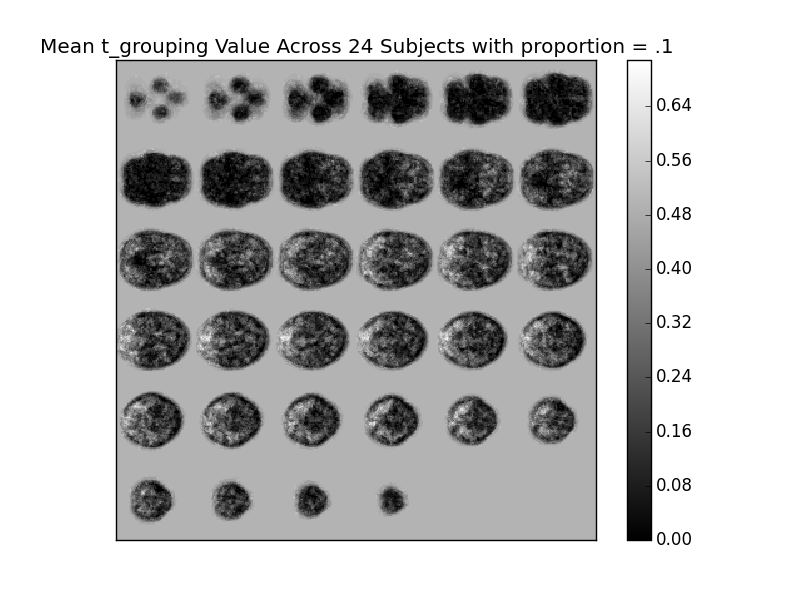
\includegraphics[width=.8\linewidth]{../images/tgroup_mean_final.png} 
	\caption{Slices from averaging the binary t-statistic masks across 
subjects. Colors indicate the proportion of subjects that identified a voxel 
as significant.}
	\label{fig:avgt}
\end{figure}

\par Additional future work could also be concerned with reproducing our 
approach for identifying actived regions on the pre-cleaned version of the 
study's data provided by the organizers of the OpenfMRI project. Those results 
could then be compared with the results from using our own pre-processing 
techniques. Since fMRI data is notoriously noisy, the different decisions made 
when cleaning the data to seperate the signal from the noise can greatly alter 
the results. So while ideally, both our pre-processed data and the 
alternatively pre-processed data would identify the same active regions, we 
acknowledge that there is a reasonably high chance that this would not be the 
case. 

\par Relating back to the issue of aggregating subjects, one great advantage 
to using the cleaned data from Ross Poldrack and the OpenfMRI project is that 
the subjects were registrated to a standard MNI anatomical template. Averaging 
clustering results across subjects would make more sense here, since the 
standard template should account for many of the differences in brain shape 
and positioning in the fMRI scanner. 
